\section{Interchange of Multirate Operations and LTI Filtering}\label{sec:p7}

\begin{enumerate}[(a)]
%----------------------------------------------------------------------------------------------
\item We have
\begin{align*}
	y
	&= D_2 A D_2 A D_2 A x \\
	&= D_2 (A D_2) (A D_2) A x \\
	&= D_2 (D_2 A(z^2)) (D_2 A(z^2)) A x \\
	&= D_2 D_2 (A(z^2) D_2) A(z^2) A x \\
	&= D_2 D_2 D_2 A(z^4) A(z^2) A x \\
	&= D_8 A(z^4) A(z^2) A(z) x \\
\end{align*}
Hence, the downsampling factor $N = 8$ and $H = A(z^4) A(z^2) A(z)$.

%----------------------------------------------------------------------------------------------
\item Figure \ref{fig:p7-2} shows the combination $H(\omega)$ if $A$ is an ideal half-band lowpass filter. The cut-off frequency is $\pm \pi/8$.
\begin{figure}[htbp]
	\centering
	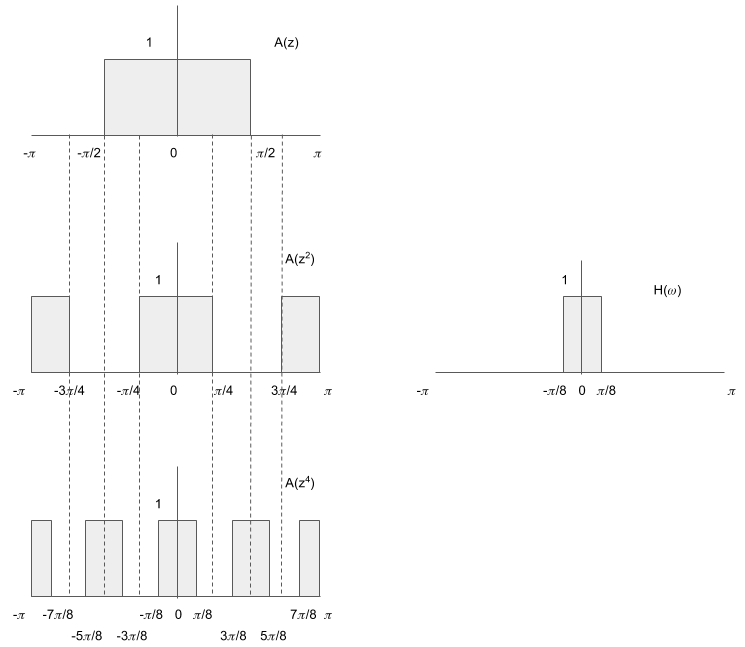
\includegraphics[width=\textwidth]{images/p7-2}
	\caption{Sketch of the low pass filters and their combination.}
	\label{fig:p7-2}
\end{figure}

%----------------------------------------------------------------------------------------------
\item Figure \ref{fig:p7-3} shows the combination $H(\omega)$ if $A$ is an ideal half-band highpass filter. The cut-off frequency is $\pm \pi/2$. The transfer function captures the highest frequency because lower ones are removed by $A(z)$.
\begin{figure}[htbp]
	\centering
	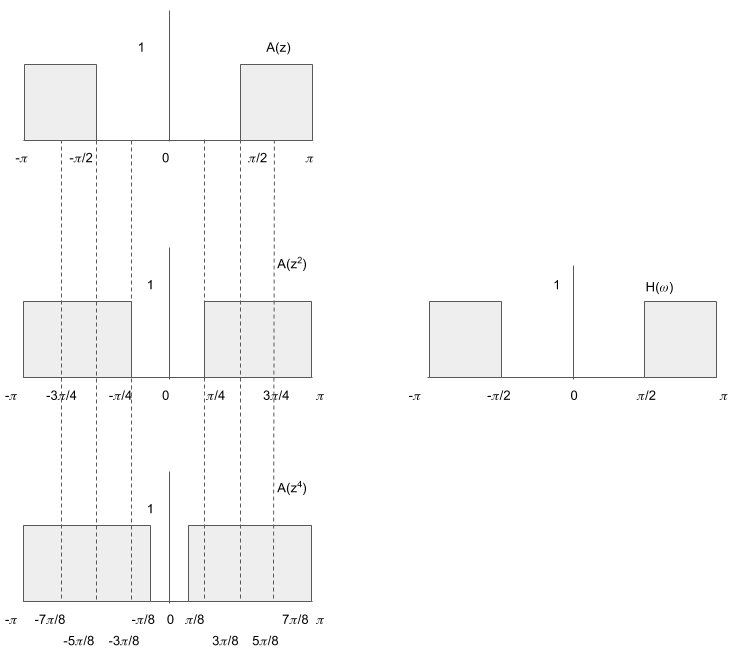
\includegraphics[width=\textwidth]{images/p7-3}
	\caption{Sketch of the high pass filters and their combination.}
	\label{fig:p7-3}
\end{figure}
\end{enumerate}